\documentclass[border=8pt]{standalone}
\usepackage[T1]{fontenc}
\usepackage{lmodern}
\usepackage{tikz}
\usetikzlibrary{shapes.geometric,fit,backgrounds}

\definecolor{ent}{HTML}{2563EB}
\definecolor{rel}{HTML}{C2410C}
\definecolor{atr}{HTML}{B45309}
\definecolor{agg}{HTML}{475569}
\definecolor{ext}{HTML}{DC2626}

\begin{document}
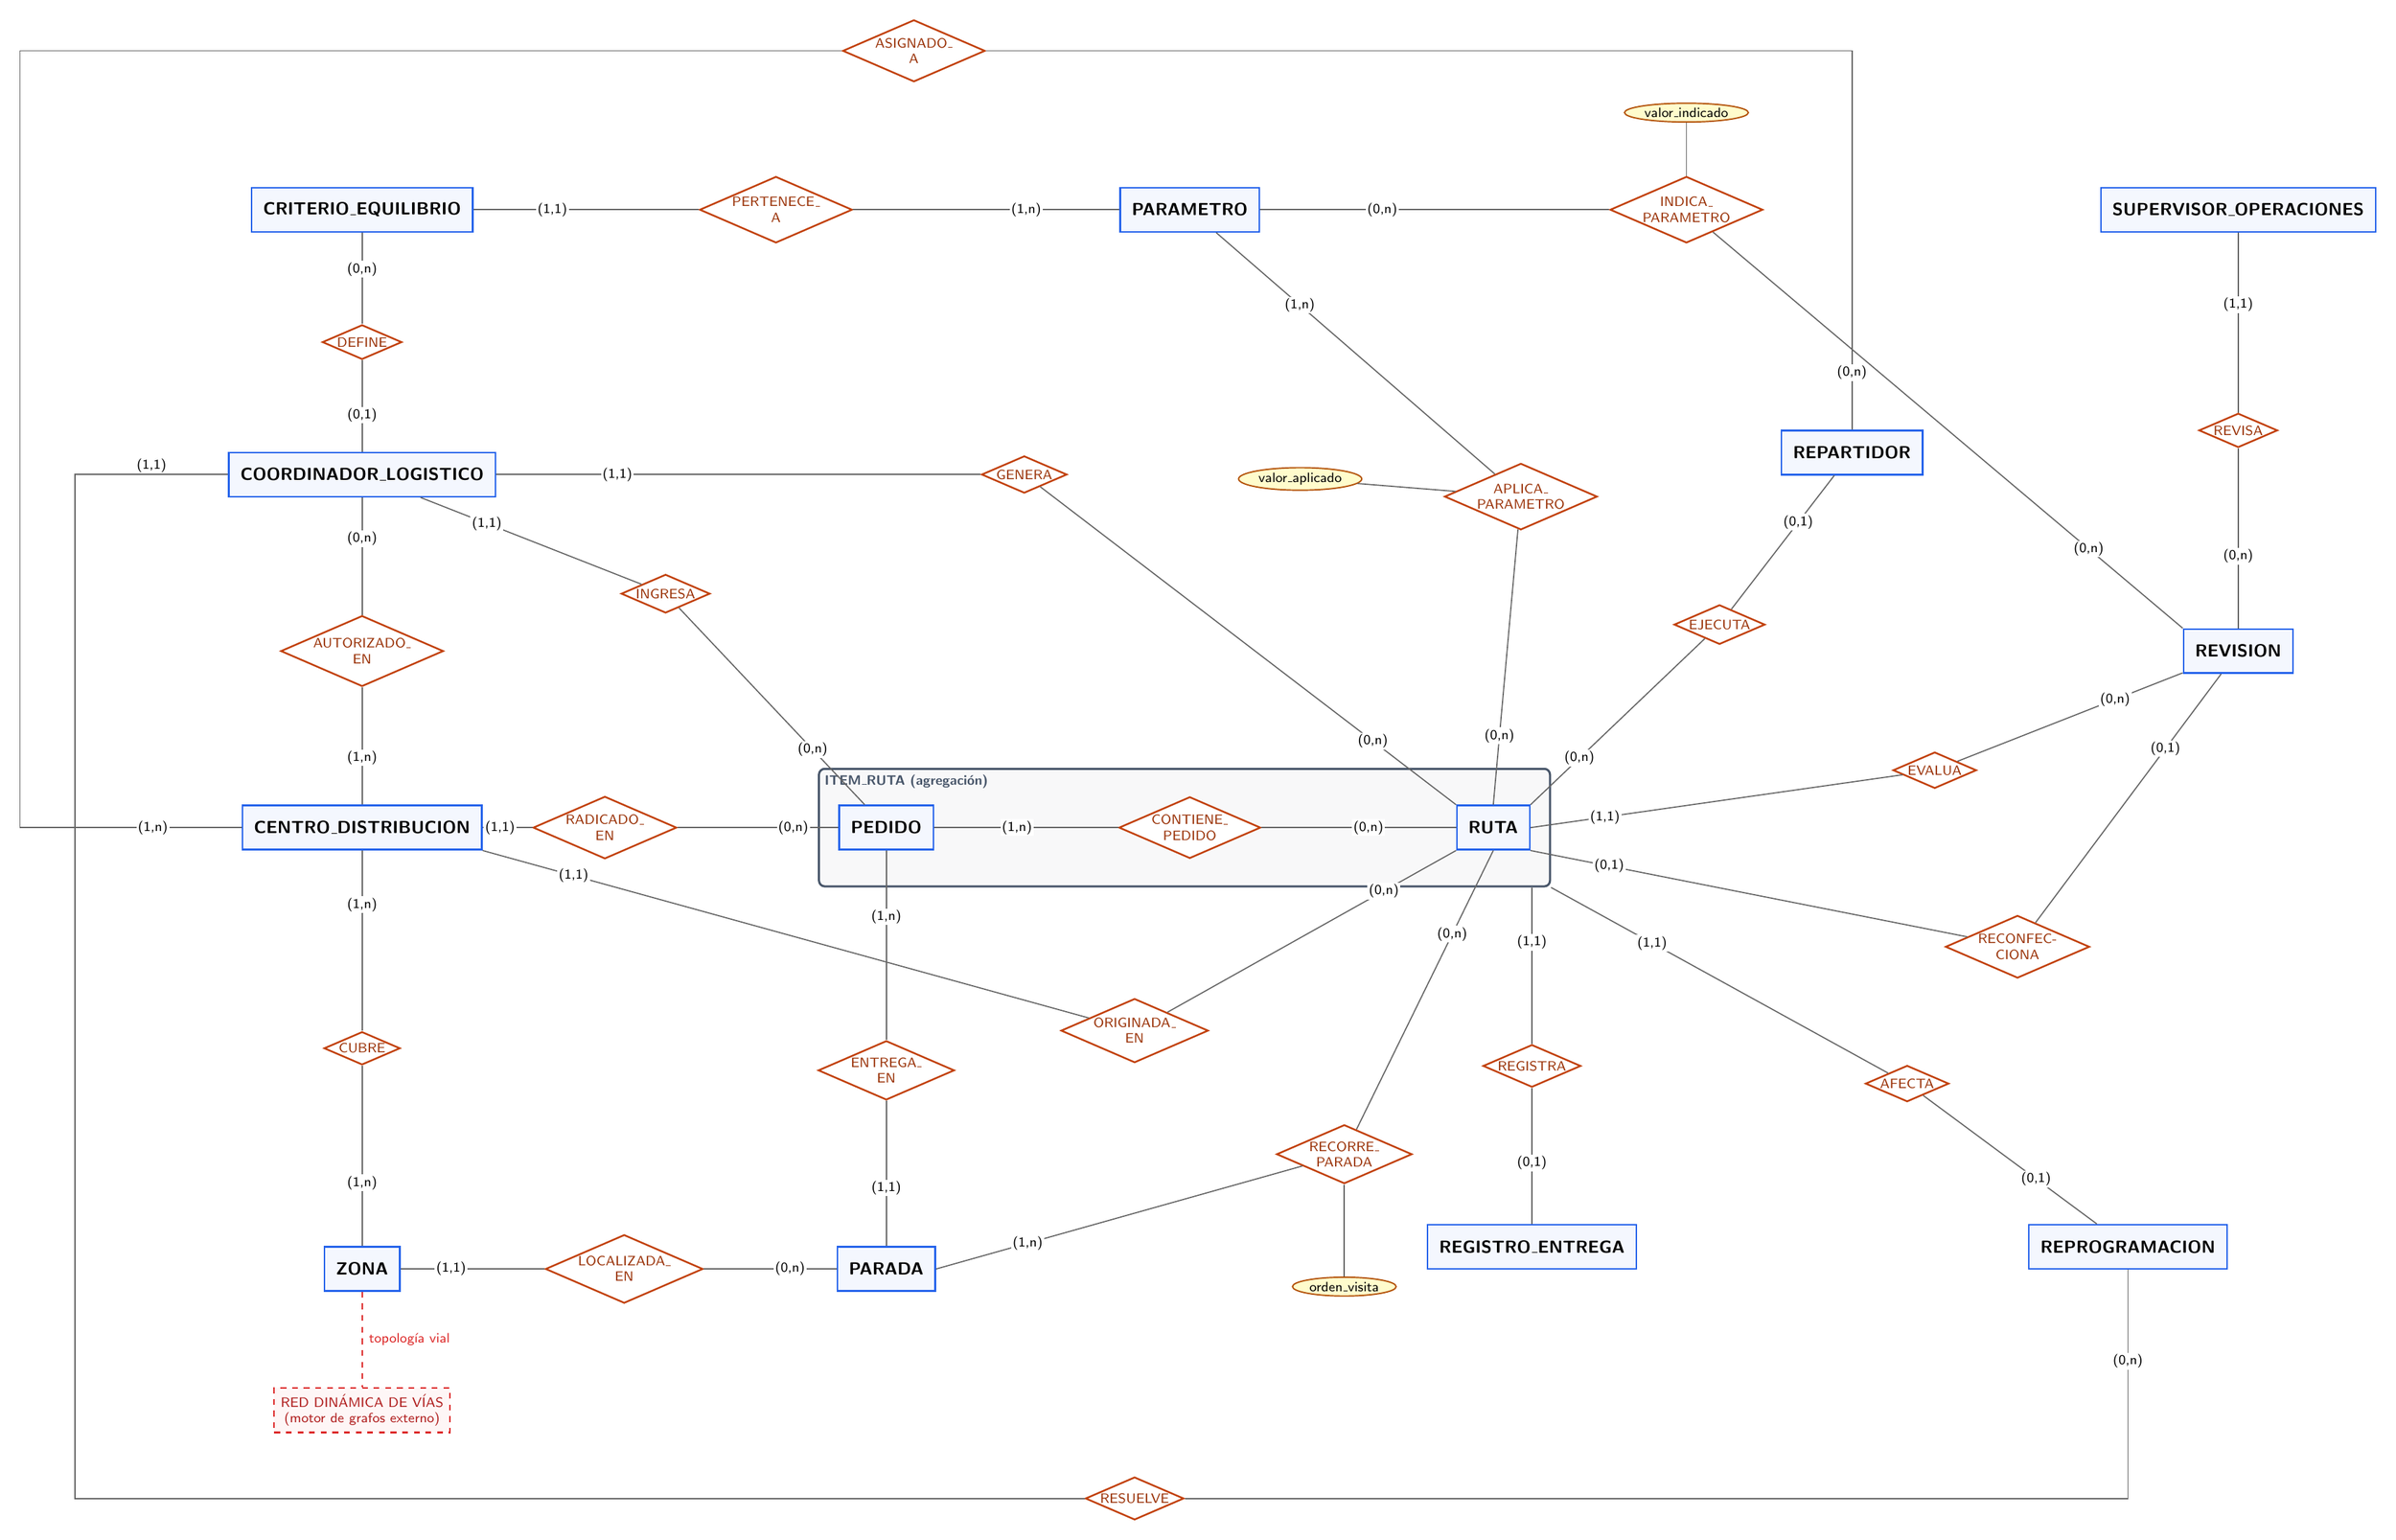
\begin{tikzpicture}[y=0.8cm,
  E/.style={rectangle,draw=ent,fill=ent!5,line width=0.9pt,font=\sffamily\small\bfseries,minimum height=0.8cm,inner xsep=6pt},
  R/.style={diamond,draw=rel,fill=white,line width=0.9pt,aspect=2.3,font=\sffamily\scriptsize,text=rel!80!black,inner sep=0.6pt,align=center},
  A/.style={ellipse,draw=atr,fill=yellow!20,line width=0.7pt,font=\sffamily\scriptsize,inner sep=1pt},
  X/.style={rectangle,draw=ext,dashed,fill=ext!4,line width=0.8pt,font=\sffamily\scriptsize,text=ext!80!black,align=center},
  C/.style={font=\sffamily\scriptsize,fill=white,inner sep=0.8pt},
  L/.style={draw=black!60,line width=0.6pt},
]

% ---------------- Entidades ----------------
\node[E] (coord) at (4,20)   {COORDINADOR\_LOGISTICO};
\node[E] (crit)  at (4,26)   {CRITERIO\_EQUILIBRIO};
\node[E] (param) at (19,26)  {PARAMETRO};
\node[E] (sup)   at (38,26)  {SUPERVISOR\_OPERACIONES};
\node[E] (rev)   at (38,16)  {REVISION};
\node[E] (rep)   at (31,20.5){REPARTIDOR};
\node[E] (centro)at (4,12)   {CENTRO\_DISTRIBUCION};
\node[E] (zona)  at (4,2)    {ZONA};
\node[E] (parada)at (13.5,2) {PARADA};
\node[E] (ped)   at (13.5,12){PEDIDO};
\node[E] (ruta)  at (24.5,12){RUTA};
\node[E] (reg)   at (25.2,2.5){REGISTRO\_ENTREGA};
\node[E] (reprog)at (36,2.5) {REPROGRAMACION};
\node[X] (red)   at (4,-1.2) {RED DIN\'AMICA DE V\'IAS\\(motor de grafos externo)};

% ---------------- Agregacion ITEM_RUTA ----------------
\node[R] (cont) at (19,12) {CONTIENE\_\\PEDIDO};
\begin{scope}[on background layer]
  \node[draw=agg,line width=1.1pt,rounded corners=3pt,fill=agg!4,fit=(ped)(cont)(ruta),inner xsep=10pt,inner ysep=14pt] (item) {};
\end{scope}
\node[font=\sffamily\scriptsize\bfseries,text=agg,anchor=north west] at (item.north west) {ITEM\_RUTA (agregaci\'on)};

% ---------------- Interrelaciones ----------------
\node[R] (aut)   at (4,16)    {AUTORIZADO\_\\EN};
\node[R] (cubre) at (4,7)     {CUBRE};
\node[R] (rad)   at (8.4,12)  {RADICADO\_\\EN};
\node[R] (ingr)  at (9.5,17.3){INGRESA};
\node[R] (def)   at (4,23)    {DEFINE};
\node[R] (pert)  at (11.5,26) {PERTENECE\_\\A};
\node[R] (gen)   at (16,20)   {GENERA};
\node[R] (apl)   at (25,19.5) {APLICA\_\\PARAMETRO};
\node[R] (ind)   at (28,26)   {INDICA\_\\PARAMETRO};
\node[R] (revisa)at (38,21)   {REVISA};
\node[R] (ejec)  at (28.6,16.6){EJECUTA};
\node[R] (eval)  at (32.5,13.3){EVALUA};
\node[R] (recon) at (34,9.3)  {RECONFEC-\\CIONA};
\node[R] (entr)  at (13.5,6.5){ENTREGA\_\\EN};
\node[R] (loc)   at (8.75,2)  {LOCALIZADA\_\\EN};
\node[R] (orig)  at (18,7.4)  {ORIGINADA\_\\EN};
\node[R] (rec)   at (21.8,4.6){RECORRE\_\\PARADA};
\node[R] (regis) at (25.2,6.6){REGISTRA};
\node[R] (afec)  at (32,6.2)  {AFECTA};
\node[R] (resu)  at (18,-3.2) {RESUELVE};
\node[R] (asig)  at (14,29.6) {ASIGNADO\_\\A};

% ---------------- Atributos de interrelaciones ----------------
\node[A] (a_ord) at (21.8,1.6)  {orden\_visita};
\node[A] (a_apl) at (21,19.9)   {valor\_aplicado};
\node[A] (a_ind) at (28,28.2)   {valor\_indicado};
\draw[L] (rec) -- (a_ord);
\draw[L] (apl) -- (a_apl);
\draw[L] (ind) -- (a_ind);

% ---------------- Aristas (cardinalidad look-across junto a cada entidad) ----------------
% AUTORIZADO_EN
\draw[L] (coord) -- node[C,pos=0.35]{(0,n)} (aut);
\draw[L] (aut) -- node[C,pos=0.6]{(1,n)} (centro);
% CUBRE
\draw[L] (centro) -- node[C,pos=0.3]{(1,n)} (cubre);
\draw[L] (cubre) -- node[C,pos=0.65]{(1,n)} (zona);
\draw[L,dashed,ext] (zona) -- node[C,right,fill=none,text=ext]{\ topolog\'ia vial} (red);
% RADICADO_EN
\draw[L] (centro) -- node[C,pos=0.35]{(1,1)} (rad);
\draw[L] (rad) -- node[C,pos=0.72]{(0,n)} (ped);
% INGRESA
\draw[L] (coord) -- node[C,pos=0.3]{(1,1)} (ingr);
\draw[L] (ingr) -- node[C,pos=0.72]{(0,n)} (ped);
% DEFINE
\draw[L] (coord) -- node[C,pos=0.4]{(0,1)} (def);
\draw[L] (def) -- node[C,pos=0.6]{(0,n)} (crit);
% PERTENECE_A
\draw[L] (crit) -- node[C,pos=0.35]{(1,1)} (pert);
\draw[L] (pert) -- node[C,pos=0.65]{(1,n)} (param);
% GENERA
\draw[L] (coord) -- node[C,pos=0.25]{(1,1)} (gen);
\draw[L] (gen) -- node[C,pos=0.8]{(0,n)} (ruta.north west);
% APLICA_PARAMETRO
\draw[L] (param) -- node[C,pos=0.3]{(1,n)} (apl);
\draw[L] (apl) -- node[C,pos=0.75]{(0,n)} (ruta.north);
% INDICA_PARAMETRO
\draw[L] (param) -- node[C,pos=0.35]{(0,n)} (ind);
\draw[L] (ind) -- node[C,pos=0.8]{(0,n)} (rev.north west);
% REVISA
\draw[L] (sup) -- node[C,pos=0.4]{(1,1)} (revisa);
\draw[L] (revisa) -- node[C,pos=0.6]{(0,n)} (rev);
% EJECUTA
\draw[L] (rep) -- node[C,pos=0.35]{(0,1)} (ejec);
\draw[L] (ejec) -- node[C,pos=0.72]{(0,n)} (ruta.north east);
% EVALUA
\draw[L] (rev) -- node[C,pos=0.3]{(0,n)} (eval);
\draw[L] (eval) -- node[C,pos=0.8]{(1,1)} (ruta.east);
% RECONFECCIONA
\draw[L] (rev) -- node[C,pos=0.3]{(0,1)} (recon);
\draw[L] (recon) -- node[C,pos=0.82]{(0,1)} (ruta.south east);
% CONTIENE_PEDIDO
\draw[L] (ruta) -- node[C,pos=0.45]{(0,n)} (cont);
\draw[L] (cont) -- node[C,pos=0.55]{(1,n)} (ped);
% ENTREGA_EN
\draw[L] (ped) -- node[C,pos=0.35]{(1,n)} (entr);
\draw[L] (entr) -- node[C,pos=0.6]{(1,1)} (parada);
% LOCALIZADA_EN
\draw[L] (parada) -- node[C,pos=0.35]{(0,n)} (loc);
\draw[L] (loc) -- node[C,pos=0.65]{(1,1)} (zona);
% ORIGINADA_EN
\draw[L] (centro.south east) -- node[C,pos=0.15]{(1,1)} (orig);
\draw[L] (orig) -- node[C,pos=0.75]{(0,n)} (ruta.south west);
% RECORRE_PARADA
\draw[L] (ruta.south) -- node[C,pos=0.3]{(0,n)} (rec);
\draw[L] (rec) -- node[C,pos=0.75]{(1,n)} (parada.east);
% REGISTRA (desde la agregacion)
\draw[L] (regis.north |- item.south) -- node[C,pos=0.35]{(1,1)} (regis);
\draw[L] (regis) -- node[C,pos=0.55]{(0,1)} (reg);
% AFECTA (desde la agregacion)
\draw[L] (item.south east) -- node[C,pos=0.3]{(1,1)} (afec);
\draw[L] (afec) -- node[C,pos=0.65]{(0,1)} (reprog);
% RESUELVE (recorrido por el borde inferior)
\draw[L] (coord.west) -- node[C,pos=0.5,above]{(1,1)} (-1.2,20) -- (-1.2,-3.2) -- (resu.west);
\draw[L] (resu.east) -- (36,-3.2) -- node[C,pos=0.6]{(0,n)} (reprog.south);
% ASIGNADO_A (recorrido por el borde superior)
\draw[L] (rep.north) -- node[C,pos=0.15]{(0,n)} (31,29.6) -- (asig.east);
\draw[L] (asig.west) -- (-2.2,29.6) -- (-2.2,12) -- node[C,pos=0.6]{(1,n)} (centro.west);

\end{tikzpicture}
\end{document}
